\documentclass[french]{RMcv}
%
\hypersetup{%
    hidelinks,%
    colorlinks=false,%
    pdfauthor={Riccardo Milani},%
    pdftitle={CV Milani},%
    pdfdisplaydoctitle=true,%
    %pdfsubject={CV},
    pdfkeywords=CV,%
    %pdfpagemode=FullScreen,%
    %pdfmenubar=false,%
    %pdftoolbar=false,%
    pdflang=fr-FR,%
    pdfcreator=LaTeX,%
}

\renewcommand\intracvevent{4pt} % Spacing between a cvevent and the previous object. Default: 6pt
%\renewcommand\intercvevent{4pt} % Spacing between first line and bullet point of a cvevent. Default: 6pt

\title{CV - Fra}

\newif\ifcvtitle
\newif\ifcvsubtitle
\cvtitlefalse
\cvsubtitlefalse

%============================================================================%
%
%
%
%  DOCUMENT CONTENT
%
%
%
%============================================================================%
\begin{document}

%---------------------------------------------------------------------------------------
%  TITLE HEADLINE
%----------------------------------------------------------------------------------------
\vspace{-20.55pt}

\cvhead{CV}

\vspace{2px}
\center{%
 \ifcvtitle{Ing\'enieur en Math\'ematiques Appliqu\'ees$\cdot$} \fi%
 Français, Italien $\cdot$ %\faFlag~
 15/01/1991 $\cdot$ %
 Paris $\cdot$ %
 \href{mailto:ricc.milani@gmail.com}{\textcolor{sectcol}{\textbf{ricc.milani@gmail.com}}} $\cdot$ %\faEnvelope
 {+33 7 83 93 34 47} $\cdot$ %\faPhone or \faMobilePhone\footnotesize
 \textcolor{sectcol}{\faLinkedinSquare{\bfseries\href{https://www.linkedin.com/in/milanir}{/in/milanir}}} $\cdot$ %
 \faGithub\href{https://github.com/RiMillo}{/RiMillo}% $\cdot$ %
}
\vspace{2px}
\center{\huge{\textbf{\textcolor{sectcol}{%
% Title
\ifcvtitle%
  PhD in Applied Mathematics / CFD%
\else%
  Ing\'enieur en Math\'ematiques Appliqu\'ees%
\fi
}}}}%
%\vspace{-2px}
% ================
% Subtitle
\ifcvsubtitle%
  \center{\large{\textcolor{bgcol}{Starting summer/fall 2017}}}%
\else%
  \vspace*{2px}
\fi
\vspace*{4px}%
% ================
\vspace{4px}%
%
%----------------------------------------------------------------------------------------
%  HEADER IMAGE
%----------------------------------------------------------------------------------------

%\begin{figure}[H]
%\begin{flushright}
  %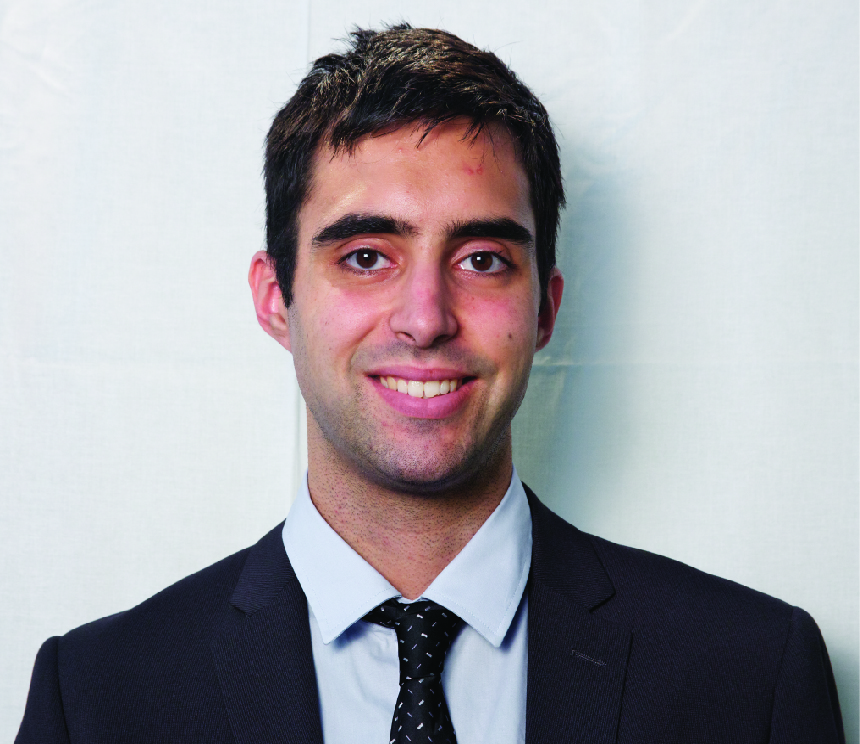
\includegraphics[trim= 320 130 460 210,clip,width=0.2\linewidth]{Foto_Smart.jpg}  %trimming relative to image size!
    %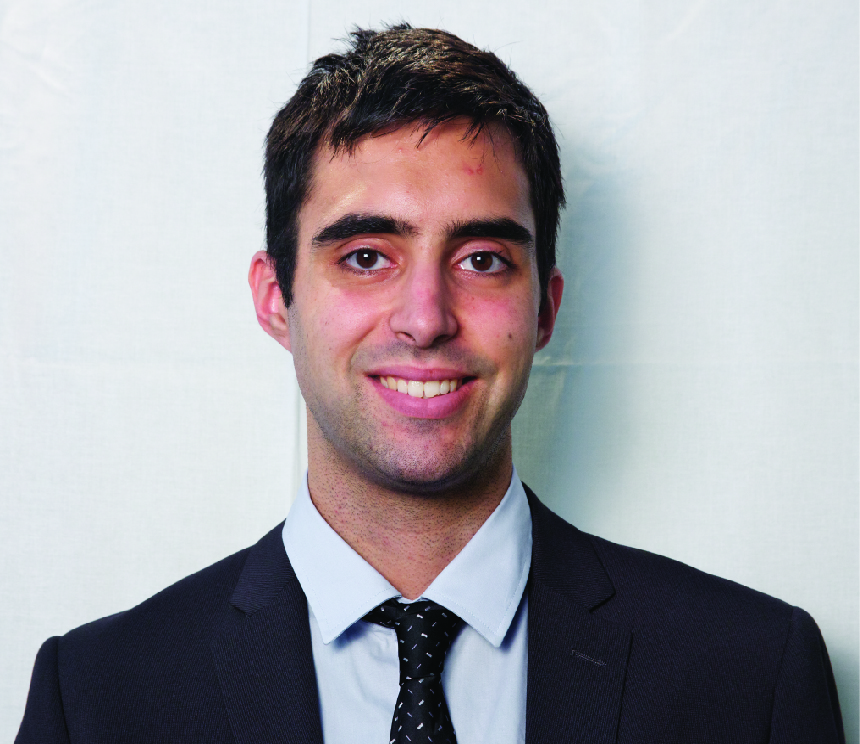
\includegraphics[width=0.2\linewidth]{Foto_Smart.jpg}
%\end{flushright}
%\end{figure}

%---------------------------------------------------------------------------------------
%  QR CODE (optional)
%----------------------------------------------------------------------------------------
%\vspace{-136pt}
%\hspace{0.75\linewidth}
%
\includegraphics[width=103pt]{qrcode}
%\normalsize
%\vspace{88pt}

%---------------------------------------------------------------------------------------
%  META SECTION
%----------------------------------------------------------------------------------------

%\vspace{-114pt}

%\metasection{Status:}{M.Sc. Digital Media, IT Consultant at We4IT Bremen}
%\metasection{Fields:}{Project Management, Software Development, Scrum, Usability}
%\metasection{Prefers:}{JS, Java, XPages, Flex / AIR, Processing, Git, Eclipse}
%\metasection{Activities:}{Global Game Jam, Sound Engineering, Blender, Martial Arts}

%\vspace{6pt}

%---------------------------------------------------------------------------------------
%  SUMMARAY (optional)
%----------------------------------------------------------------------------------------

%\cvsection{Summary}\\
%Digital media graduate with four years project experience in the field of technology based assessment. Specialized in development of test-scenario engines and innovative, rich media item formats. Master studies focused on teams from different disciplines and cultural backgrounds on solutions for complex problems.  Prior knowledge has been collected in he field of usability / accessibility during bachelor studies.\\

%============================================================================%
%
%  CV SECTIONS AND EVENTS (MAIN CONTENT)
%
%============================================================================%

%---------------------------------------------------------------------------------------
%  EDUCATION SECTION
%--------------------------------------------------------------------------------------
\cvsection{Formation}

\cvevent{depuis 2017}%
        {Doctorant en Math\'ematiques Appliqu\'ees}%
        {\'Ecole des Ponts ParisTech - EDF R\&D}%
        {Sch\'emas de discr\'etisation \emph{Compatible Discrete Operator} pour les \'equations de Navier--Stokes instationnaires d'un fluide incompressible}%
        {Directeur : Ern Alexandre (CERMICS, INRIA); Encadrant : Bonelle J\'er\^ome (EDF R\&D)}

\cvevent{2015 - 2017}%
        {Master 2 en Ing\'enierie}%
        {Politecnico di Milano}%
        {\emph{Laurea Magistrale} en Ing\'enierie Math\'ematique, sp\'ecialisation: Math\'ematiques Appliqu\'ees \& Sciences Informatiques}%
        {Note: 110/110 avec mention}

%\textcolor{softcol}{\hrule}

%
\cvevent{2013 - 2017}%
        {Cycle de l'Ing\'enieur \textit{Polytechnicien}}%
        {\'Ecole polytechnique}%
        {Licence et Master 1 en Ing\'enierie}%
        {Programme d'Approfondissement : Math\'ematiques Appliqu\'ees - EDP}

%\textcolor{softcol}{\hrule}

%
\cvevent{2010 - 2015}%
        {Licence en Ing\'enierie}%
        {Politecnico di Milano}%
        {\emph{Laurea Triennale} en Ing\'enierie Math\'ematique. Note: 110/110 avec mention}%
        {\'Elu meilleur \'el\`eve de premi\`ere ann\'ee apr\`es r\'esultats du test d'admission et des examens du premier semestre (2010)}

%---------------------------------------------------------------------------------------
%  EXPERIENCE
%----------------------------------------------------------------------------------------
\cvsection{Exp\'eriences professionnelles}

%
\cvevent{09/'16-02/'17}%
        {Stage de Recherche, 6 mois}%
        {EDF R\&D, Chatou}%
        {D\'eveloppement et analyse num\'erique d'une m\'ethode \emph{Hybrid High-Order} pour la diffusion anisotrope en 3D}%
        {Int\'egration dans le code industriel \cs{} (\texttt{C}); parall\'elisation \`a l'aide de OpenMP}

%\textcolor{softcol}{\hrule}

%
\cvevent{03-08/2015}%
        {Stage de Recherche, 5 mois}%
        {US ESI R\&D, San Diego}%
        {Premiers d\'eveloppements pour une nouvelle m\'ethode de calcul rapide de la r\'eponse vibro-acoustique d'un syst\`eme}%
        {Validation avec simulations (MATLAB)}

%\textcolor{softcol}{\hrule}

%
\cvevent{08/2014}%
        {Stage d'\'et\'e, 1 mois}%
        {VTB Bank, Irkutsk}%
        {Groupe de contr\^ole des devises \'etrang\`eres}%
        {Aide \`a la pr\'eparation et \`a la validation finale de dossiers concernant contrats internationaux; gestion d'archives}

\vspace{5pt}
\begin{minipage}{.48\linewidth}
\begin{flushleft}
\cvsubsection{Comp\'etences informatiques}
\vspace{6pt}
\begin{tabular*}{1\linewidth}{l l}
&     \larrow{bgcol} \textbf{Bonne connaissance}: \texttt{C}/\texttt{C++}, OpenMP, MPI,\\[3pt]
&       \LaTeX, Unix, MATLAB, Git/SVN, \cs{}, Office\\[3pt]
&     \larrow{bgcol} \textbf{Notions de base}: Python, shell script, Fortran,\\[3pt]
&       FreeFem\texttt{++}, SALOME, Java, R
\end{tabular*}
\end{flushleft}
\end{minipage}
\hfill
\begin{minipage}{.48\linewidth}
\begin{flushright}
\cvsubsection{Langues}
\vspace{6pt}
\begin{tabular*}{1\linewidth}{l l l}
&     \larrow{bgcol} \textbf{Italien}:  &Langue maternelle\\[3pt]
&     \larrow{bgcol} \textbf{Français}: &Courant, certificat TCF, C1\\[3pt]
&     \larrow{bgcol} \textbf{Anglais}:  &Courant, certificat FCE, B2\\[3pt]
&     \larrow{bgcol} \textbf{Russe}:    &Notions\\[3pt]
\end{tabular*}
\end{flushright}
\end{minipage}

\medskip

\begin{minipage}{.48\linewidth}
\begin{flushleft}
\cvsubsection{Activit\'es extra-professionnelles}
\vspace{6pt}
\begin{tabular*}{1\linewidth}{l l}
&     \larrow{bgcol} Responsable d'un foyer \'etudiant ('15)\\[3pt]
&     \larrow{bgcol} Tr\'esorier de l'AIM ('16)\\[3pt]
&     \larrow{bgcol} Doctorant r\'ef\'erent pour EDF-MFEE ('18-'20)\\[3pt]
&     \larrow{bgcol} Running (marathon de Paris '19)\\[3pt]
\end{tabular*}
\end{flushleft}
\end{minipage}
\hfill
\begin{minipage}{.48\linewidth}
\begin{flushright}
\cvsubsection{Centres d'int\'er\^et et B\'en\'evolat}
\vspace{6pt}
\begin{tabular*}{1\linewidth}{l l}
&     \larrow{bgcol} Camps d'\'et\'e (Kenya '10, '11; Rwanda '17)\\[3pt]
&     \larrow{bgcol} Membre active de l'association Smileland, qui\\[3pt]
&       soutient un village au Congo\\[3pt]
&     \larrow{bgcol} Professeur d'italien pour les r\'efugi\'es ('15)\\[3pt]
\end{tabular*}
\end{flushright}
\end{minipage}




%-------------------------------------------------------------------------------------------------
%  ARTIFICIAL FOOTER (fancy footer cannot exceed linewidth)
%--------------------------------------------------------------------------------------------------

\null
\vspace*{\fill}
%\hspace{-0.25\linewidth}\colorbox{bgcol}{\makebox[1.5\linewidth][c]{\mystrut \small \textcolor{white}{www.jankuester.com} $\cdot$ \textcolor{white}{github.com/jankapunkt}}}




%============================================================================%
%
%
%
%  DOCUMENT END
%
%
%
%============================================================================%
\end{document}
